\documentclass[conference, a4paper]{IEEEtran}
\IEEEoverridecommandlockouts

\usepackage[utf8]{inputenc} 
\usepackage[T1]{fontenc}
\usepackage{graphicx}
\usepackage[super]{nth}
\usepackage{booktabs}
\usepackage{caption}
\usepackage{subcaption}
\usepackage[hyphens]{url}
\usepackage{hyperref}
\hypersetup{breaklinks=true}
\usepackage{xcolor}
\usepackage{balance}
\usepackage{cite}
\usepackage{multirow}
\usepackage{array}
\usepackage[cmex10]{amsmath}
\usepackage{amsfonts}
\usepackage{diagbox}
\usepackage{makecell}
\usepackage{placeins}
\usepackage{stfloats} % Çift sütunlu figürleri düzgün yerleştirmek için KRİTİK PAKET

\hyphenation{op-tical net-works semi-conduc-tor}
\setlength{\textfloatsep}{10pt} % Figür ile metin arası boşluk
\setlength{\dbltextfloatsep}{12pt} % Çift sütun figür ile metin arası boşluk

\begin{document}

\title{High-Performance GPU Acceleration of FMCW Radar Signal Processing and 2D CA-CFAR Detection}

\author{
\IEEEauthorblockN{Bahadır Çeliktaş}
\IEEEauthorblockA{
\textit{ASELSAN A.Ş.}\\
Ankara, Türkiye \\
bahadirce@aselsan.com \\
ORCID: 0009-0008-5586-9922}
\and
\IEEEauthorblockN{Eşrefhan Kadıoğlu}
\IEEEauthorblockA{
\textit{ASELSAN A.Ş.}\\
Ankara, Türkiye \\
esrefhankadi@aselsan.com \\
ORCID: 0009-0000-8607-7081}
\and
\IEEEauthorblockN{Onur Göksel}
\IEEEauthorblockA{
\textit{ASELSAN A.Ş.}\\
Ankara, Türkiye \\
onurgoksel@aselsan.com \\
ORCID: 0000-0002-4152-3196}
}

\maketitle

\begin{abstract}
Modern FMCW radar systems generate large-scale high-resolution data requiring computationally intensive signal processing. 
Range–Doppler spectrum generation via multi-dimensional FFT operations and subsequent 2D CA-CFAR detection introduce significant latency when executed on CPU architectures. 
This paper presents a unified GPU-accelerated radar signal processing pipeline integrating FFT-based spectral processing and adaptive CFAR detection. 
Multiple CPU and CUDA-based implementations are systematically compared, including naive, SIMD-optimized, summed-area-table-based, and shared-memory-optimized kernels. 
Experimental results demonstrate speedups of up to $71\times$ over baseline CPU implementations while preserving numerical accuracy and detection performance. 
A detailed bandwidth and bottleneck analysis shows that once computation is accelerated, PCIe data transfer becomes the dominant constraint.
\end{abstract}

\begin{IEEEkeywords}
FMCW Radar, GPU Acceleration, CUDA, FFT, CA-CFAR, High-Performance Computing
\end{IEEEkeywords}

\section{Introduction}
Frequency Modulated Continuous Wave (FMCW) radar systems determine target range and velocity through multi-stage digital signal processing. The Range–Doppler map is obtained via sequential FFT operations along fast-time and slow-time dimensions, followed by adaptive detection using Constant False Alarm Rate (CFAR) algorithms. Furthermore, the real-time generation of these high-resolution radar representations is increasingly critical, as they serve as essential inputs for advanced downstream tasks, such as deep learning-based automotive object recognition \cite{9249018}.

As radar resolution increases, matrix sizes frequently exceed $2048 \times 2048$, making real-time processing challenging on CPU architectures. Although multi-threading and SIMD-based optimizations provide partial improvements, they remain insufficient for large-scale deployments. 

Graphics Processing Units (GPUs) offer massive data-level parallelism, enabling significant acceleration of FFT and sliding-window detection operations. This study proposes a unified GPU-accelerated FMCW radar processing pipeline and evaluates multiple optimization strategies.

\section{Related Work}

GPU-based acceleration of radar processing has been widely investigated. 
Venter \textit{et al.} \cite{venter2011} implemented CA-CFAR on GPU architectures, demonstrating substantial performance gains over CPU implementations for sliding-window detection.

Zhao \textit{et al.} \cite{zhao2023} presented a GPU-accelerated radar processing pipeline integrating Range–Doppler processing and CFAR detection using CUDA and cuFFT, emphasizing memory optimization strategies.

Liu \textit{et al.} \cite{liu2023} proposed a real-time GPU-based radar processing framework for MIMO systems, highlighting architectural considerations for sustaining real-time throughput.

GPU acceleration has also been applied to Range–Doppler algorithms in FMCW-based SAR systems, where kernel fusion and pinned memory reduce data-transfer overhead \cite{jung2023}.

Despite these advances, few works provide a unified framework that systematically compares multiple CPU and GPU implementations of both FFT and 2D CA-CFAR under identical experimental conditions.

\section{Methodology}

This study presents a unified FMCW radar signal processing framework integrating 2D FFT-based range–Doppler estimation with CA-CFAR detection, accelerated using GPU architectures. The objective is to reduce computational complexity for large radar data cubes and enable real-time processing performance.

\subsection{FMCW Signal Model}

An FMCW radar transmits a linear frequency-modulated (LFM) chirp signal expressed as \cite{richards2014}:

\begin{equation}
s_t(t) = A \exp \left( j 2\pi \left( f_c t + \frac{B}{2T} t^2 \right) \right)
\end{equation}

where $f_c$ is the carrier frequency, $B$ is the sweep bandwidth, and $T$ is the chirp duration.

The received echo from a target at range $R$ is delayed by $\tau = \frac{2R}{c}$ and given by:

\begin{equation}
s_r(t) = A \exp \left( j 2\pi \left( f_c (t-\tau) + \frac{B}{2T} (t-\tau)^2 \right) \right)
\end{equation}

After dechirping, the intermediate beat frequency becomes:

\begin{equation}
f_b = \frac{B}{T} \tau
\end{equation}

Thus, the target range is estimated as \cite{richards2014}:

\begin{equation}
R = \frac{cT}{2B} f_b
\end{equation}

\subsection{Range–Doppler Processing}

Range and velocity estimation are performed using two-dimensional FFT operations across the fast-time and slow-time dimensions \cite{richards2014}. The discrete Fourier transform (DFT) applied in the range dimension is defined as:

\begin{equation}
X(k) = \sum_{n=0}^{N-1} x(n) e^{-j 2\pi kn/N}
\end{equation}

where $N$ represents the number of ADC samples per chirp.

Subsequently, Doppler processing is performed across $M$ chirps:

\begin{equation}
S(k,m) = \sum_{l=0}^{M-1} X(k,l) e^{-j 2\pi ml/M}
\end{equation}

The resulting 2D FFT produces the range–Doppler map. Since each FFT stage has computational complexity $O(N \log N)$, the overall processing cost becomes significant for large grids. GPU acceleration of FFT-based radar algorithms has been shown to provide substantial performance improvements in similar radar systems \cite{jung2023,zhao2023,liu2023}.

\subsection{CA-CFAR Detection}

To detect targets within the range–Doppler map, a two-dimensional Cell-Averaging Constant False Alarm Rate (CA-CFAR) detector is employed. The CA-CFAR algorithm computes an adaptive threshold using surrounding reference cells \cite{venter2011}.

For each Cell Under Test (CUT), the threshold is calculated as:

\begin{equation}
T = \alpha \cdot \frac{1}{N_r} \sum_{i=1}^{N_r} P_i
\end{equation}

where $N_r$ denotes the number of reference cells, $P_i$ represents the power of the $i$-th reference cell, and $\alpha$ is a scaling factor determined by the desired probability of false alarm.

Naive implementations require repeated summation over sliding windows, resulting in high computational cost. To reduce this complexity, a Summed-Area Table (SAT) approach is adopted \cite{crow1984}. The SAT enables constant-time window summation, significantly reducing the computational overhead of the CFAR stage. GPU implementations of CA-CFAR have demonstrated substantial acceleration compared to CPU-based solutions \cite{venter2011}.

\subsection{Processing Pipeline}

The complete radar signal processing pipeline consists of the following stages:

\begin{enumerate}
    \item ADC Data Acquisition
    \item Range FFT (Fast-Time FFT)
    \item Doppler FFT (Slow-Time FFT)
    \item Matrix Transpose
    \item 2D CA-CFAR Detection
\end{enumerate}

The transpose stage is included to optimize memory access patterns, particularly for GPU architectures where coalesced memory access is critical for performance \cite{liu2023,zhao2023}.

\subsection{CPU Implementations}

The CPU baseline implementations include:

\begin{itemize}
    \item Multi-threaded FFT execution
    \item SIMD vectorization
    \item SAT-based CFAR optimization
\end{itemize}

These techniques aim to exploit instruction-level and thread-level parallelism.

\subsection{GPU Implementations}

CUDA-based implementations are developed to leverage massive parallelism and high memory bandwidth:

\begin{itemize}
    \item Shared-memory optimized FFT kernels
    \item Custom transpose kernels for coalesced access
    \item Fully parallel GPU-based SAT-CFAR implementation
    \item Vendor-optimized FFT baseline for comparison
\end{itemize}

Prior studies demonstrate that GPU-accelerated radar signal processing pipelines significantly outperform CPU-based systems in real-time scenarios \cite{jung2023,zhao2023,liu2023}. The proposed framework integrates FMCW modeling, 2D FFT processing, and SAT-accelerated CA-CFAR into a unified GPU-optimized architecture suitable for high-resolution real-time radar applications.

% --- FİGÜRLER SAYFANIN BAŞINA DÜŞMESİ İÇİN BURADA ---
\begin{figure*}[!t]
    \centering
    \begin{subfigure}[b]{0.48\textwidth}
        \centering
        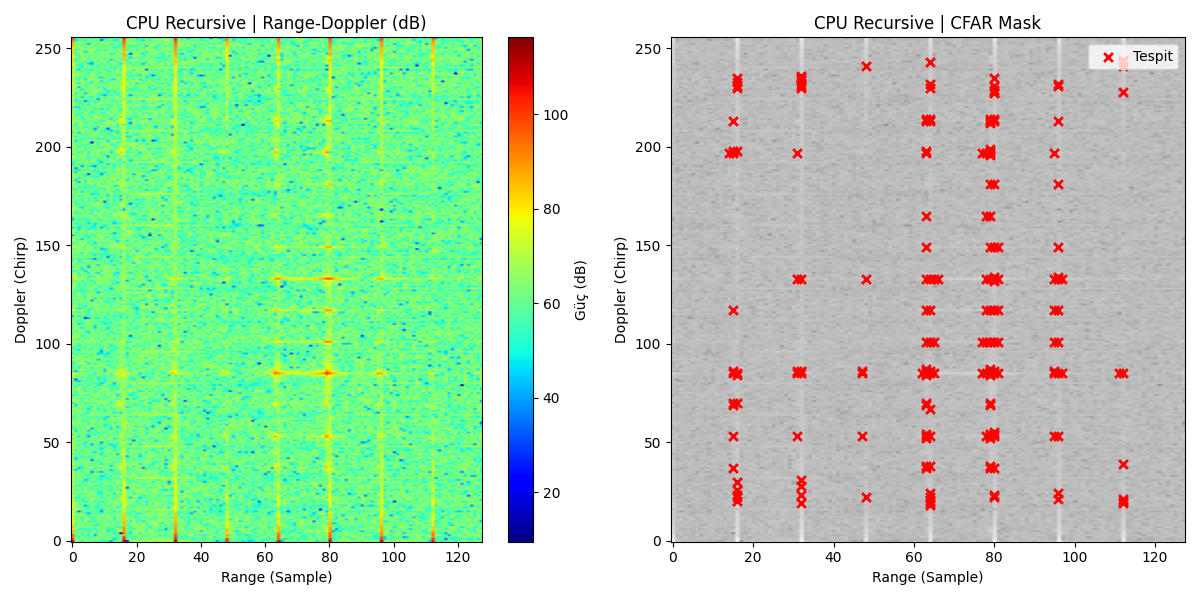
\includegraphics[width=0.95\linewidth]{CPU Recursive.png}
        \caption{CPU Recursive OpenMP}
        \label{fig:real_cpu_rec}
    \end{subfigure}
    \hfill
    \begin{subfigure}[b]{0.48\textwidth}
        \centering
        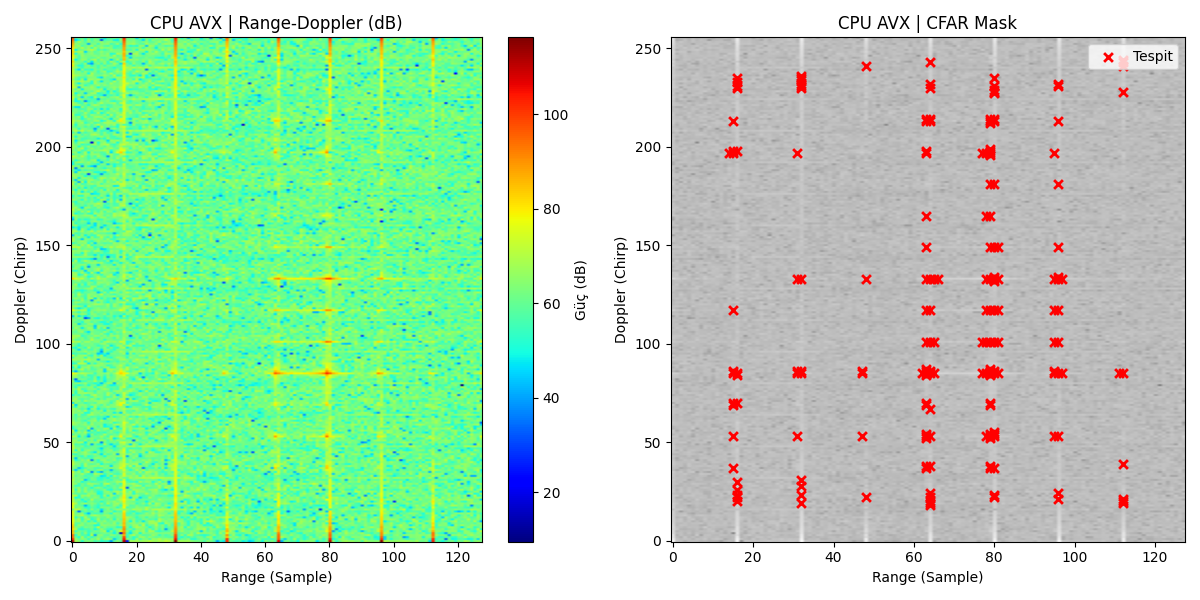
\includegraphics[width=0.95\linewidth]{CPU AVX.png}
        \caption{CPU AVX OpenMP}
        \label{fig:real_cpu_avx}
    \end{subfigure}
    
    \vspace{0.2cm}
    
    \begin{subfigure}[b]{0.48\textwidth}
        \centering
        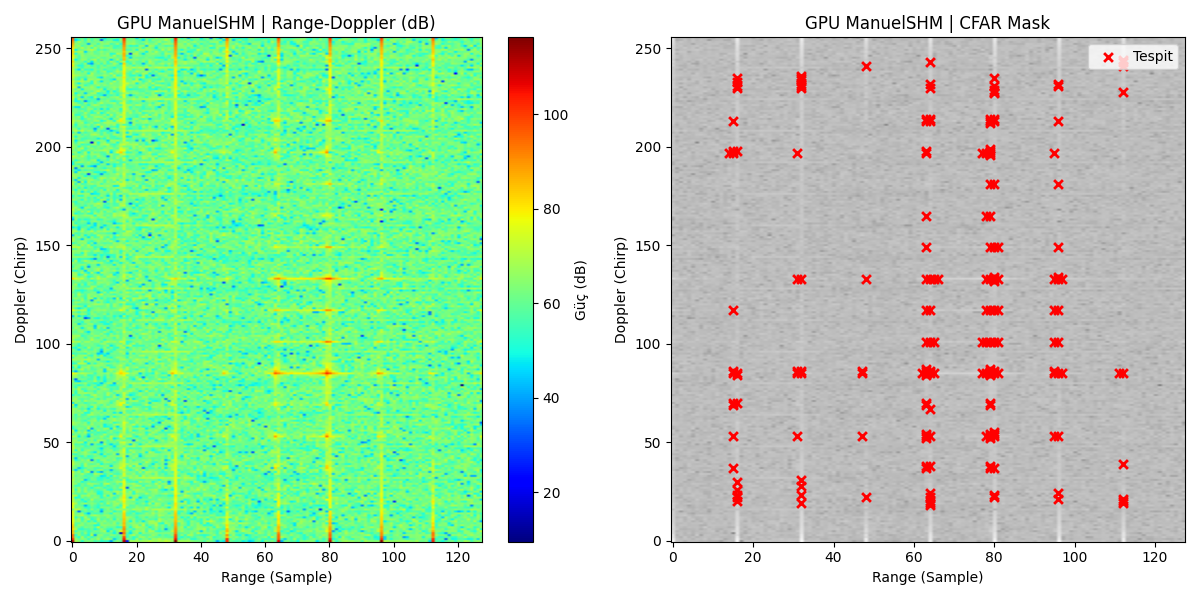
\includegraphics[width=0.95\linewidth]{GPU ManuelSHM.png}
        \caption{GPU Manual Shared Mem}
        \label{fig:real_gpu_shm}
    \end{subfigure}
    \hfill
    \begin{subfigure}[b]{0.48\textwidth}
        \centering
        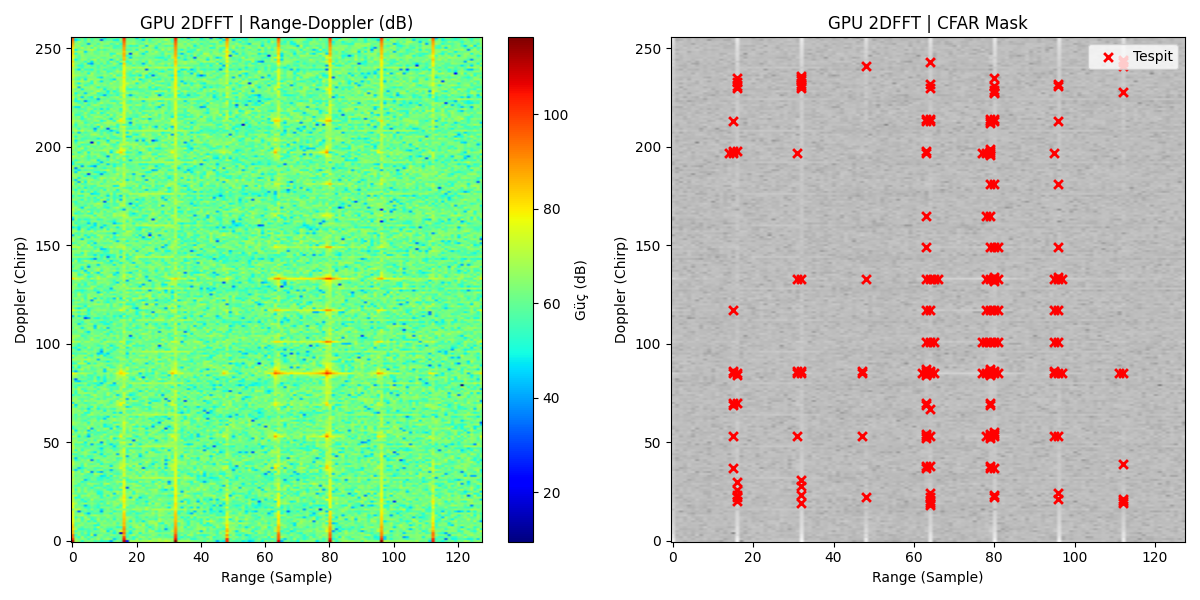
\includegraphics[width=0.95\linewidth]{GPU 2DFFT.png}
        \caption{GPU 2D\_FFT}
        \label{fig:real_gpu_2dfft}
    \end{subfigure}
    \caption{Visual comparison of Range-Doppler maps (left panel) and CA-CFAR detection masks (right panel, red crosses indicate detections) generated by different implementations using the real automotive radar dataset. All methods produce visually identical detection results, confirming the numerical precision of the GPU-accelerated algorithms.}
    \label{fig:real_data_visuals}
\end{figure*}

\begin{figure*}[!t]
    \centering
    \begin{subfigure}[b]{0.45\textwidth} 
        \centering
        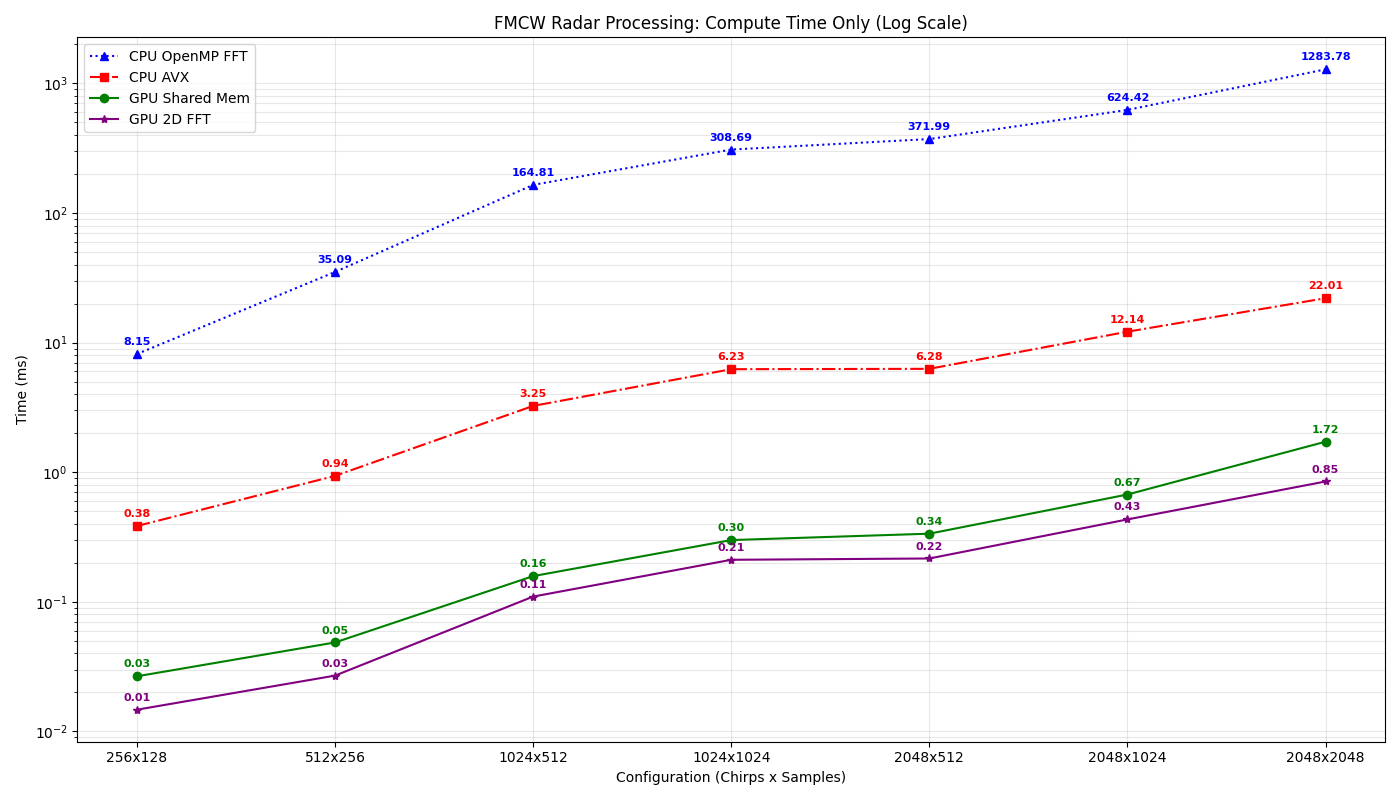
\includegraphics[width=\linewidth]{benchmark_fft_compute_time.png}
        \caption{FFT computation time (log scale)}
        \label{fig:fft_time_synthetic}
    \end{subfigure}
    \hfill
    \begin{subfigure}[b]{0.45\textwidth}
        \centering
        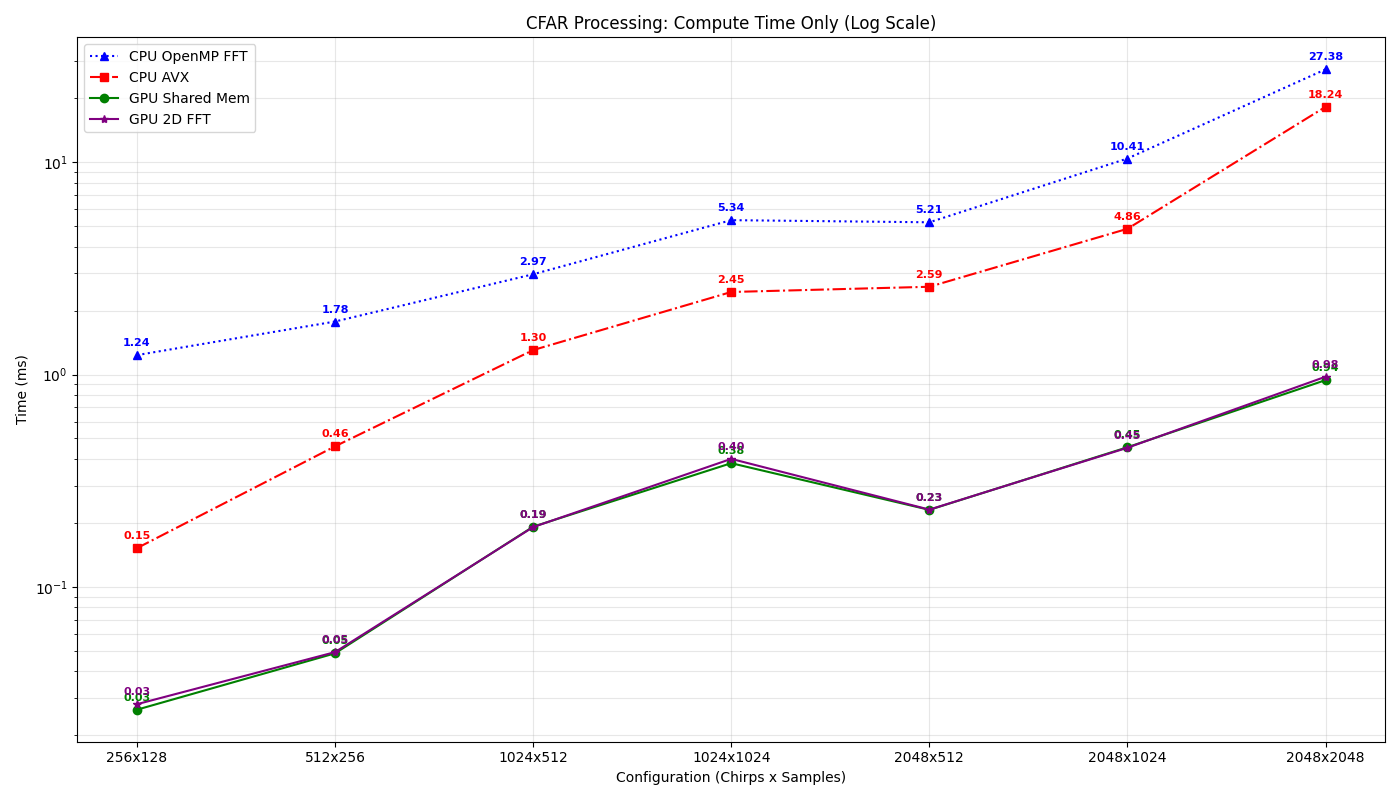
\includegraphics[width=\linewidth]{benchmark_cfar_compute_time.png}
        \caption{CFAR execution time (log scale)}
        \label{fig:cfar_time_synthetic}
    \end{subfigure}
    
    \vspace{0.2cm}

    \begin{subfigure}[b]{0.45\textwidth}
        \centering
        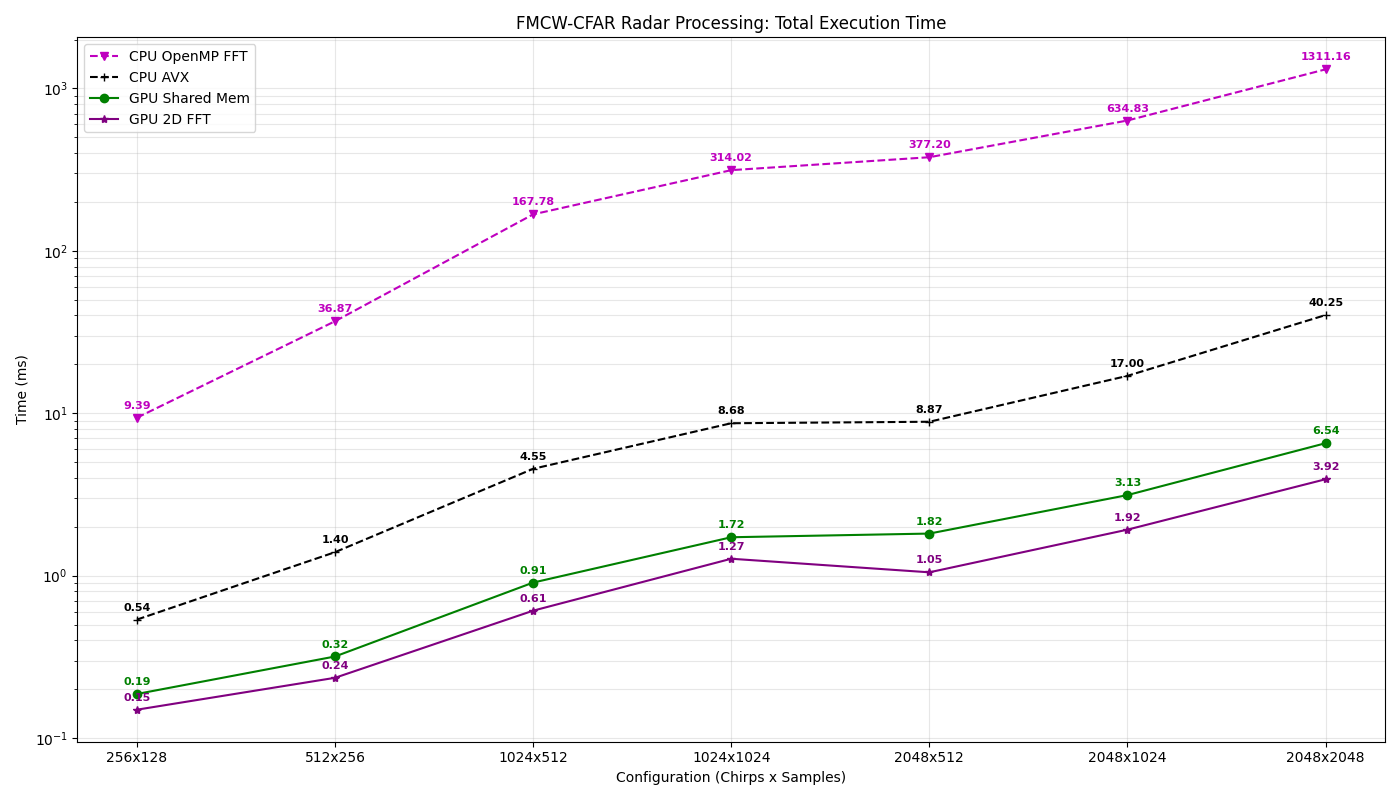
\includegraphics[width=\linewidth]{benchmark_total_time.png}
        \caption{Total execution time (log scale)}
        \label{fig:total_time_synthetic_c}
    \end{subfigure}

    \caption{Performance scaling analysis using synthetic data with varying (Chirp $\times$ Sample) grid dimensions. The GPU implementations demonstrate superior scalability and consistently lower execution times compared to CPU-based approaches as the data size increases significantly. Note the logarithmic scale on the y-axis.}
    \label{fig:synthetic_performance}
\end{figure*}
% ----------------------------------------------------

\section{Experimental Setup}

Experiments were conducted on NVIDIA RTX 4090 GPUs. Radar grids up to $2048 \times 2048$ were evaluated. 

Performance metrics include:

\begin{itemize}
    \item Kernel Compute Time
    \item Total Execution Time
    \item Effective Memory Bandwidth
    \item Speedup Factor
    \item Probability of Detection ($P_d$)
    \item Empirical False Alarm Rate ($P_{fa}$)
    \item RMSE for numerical validation
\end{itemize}

\section{Results and Discussion}

GPU cuFFT achieved up to $71\times$ speedup over recursive CPU FFT. Shared-memory optimized kernels approached vendor-level performance. GPU SAT-CFAR achieved up to $27\times$ acceleration over naive CPU implementations while maintaining detection accuracy. 

To validate the proposed implementations in real-world scenarios, experiments were conducted using an automotive raw ADC radar dataset\cite{xm40-jx59-22}. The execution times for FMCW and CFAR processing stages across different CPU and GPU methods are detailed in Table \ref{tab:real_data_performance}. As shown in Fig. \ref{fig:real_data_visuals}, all implementations yield visually consistent Range-Doppler spectra and detection masks. This verifies that the significant speedups achieved by GPU acceleration do not compromise the numerical accuracy required for reliable target detection in practical applications.

\begin{table}[htbp]
 \centering
 \caption{Execution Times on Real Automotive Radar Dataset}
 \renewcommand{\arraystretch}{1.2}
  \resizebox{\columnwidth}{!}{
  \begin{tabular}{l|ccc}
  \toprule
\textbf{Implementation} & \textbf{FMCW (ms)} & \textbf{CFAR (ms)} & \textbf{TOTAL (ms)} \\
\midrule
CPU Recursive FFT OpenMP & 8.433700 & 1.113400 & 9.547100 \\
CPU AVX FFT OpenMP & 0.343600 & 0.157100 & 0.500700 \\
GPU Manual FFT Shared Mem& 0.026781 & 0.027558 & 0.188918 \\
GPU 2D\_FFT & 0.014746 & 0.026387 & 0.133174 \\
\bottomrule
\end{tabular}
}
\label{tab:real_data_performance}
\end{table}

To systematically evaluate the scalability of the proposed algorithms beyond the fixed size of the real dataset, synthetic FMCW radar data was generated with varying grid dimensions, ranging from $256 \times 128$ to $2048 \times 2048$. Using synthetic data allows for a controlled analysis of computational bottlenecks as the matrix size increases. 

Figure \ref{fig:synthetic_performance} illustrates the computational time scaling behavior for FFT and total execution under varying grid dimensions. As observed in Fig. \ref{fig:total_time_synthetic_c}, the CPU-based OpenMP implementation exhibits an exponential increase in execution time, exceeding 1300 ms for the largest grid size, rendering it unsuitable for real-time applications. While AVX vectorization provides a significant reduction in processing time, the GPU-accelerated approaches consistently outperform all CPU variants. Specifically, the GPU 2D FFT and Shared Memory kernels maintain compute times well below 10 ms even at the massive $2048 \times 2048$ resolution, demonstrating excellent scalability.

As compute time decreased below a few milliseconds on the GPU, detailed profiling revealed that PCIe data transfer latency from the host to the device became the dominant bottleneck in the overall pipeline. To mitigate this effect, pinned memory allocation via \texttt{cudaMallocHost} was utilized during the 2D-FFT stage, which enables higher transfer bandwidth by preventing page-swapping overhead. However, it is worth noting that in integrated System-on-Chip (SoC) architectures where the CPU and GPU share the same physical RAM, this PCIe bottleneck is inherently eliminated. In such on-chip systems, the unified memory architecture allows for zero-copy data access, which would further enhance the real-time throughput of the proposed radar pipeline.

\FloatBarrier

\section{Conclusion}

This study presented a unified GPU-accelerated FMCW radar signal processing and CFAR detection framework.
Significant acceleration was achieved while maintaining numerical accuracy and detection integrity.
Future optimizations should focus on overlapping data transfers and kernel execution to mitigate PCIe bottlenecks.

%\balance

\bibliographystyle{IEEEtran}
\bibliography{references}

\end{document}